% Chapter 2: Related Work

\section{Related work}

\subsection{Internet of things}

\subsection{Industry 4.0}
%Industry 4.0 definition
Lasi argues that the term Industry 4.0 was coined beforehand as a planned fourth industrial revolution \cite{lasi}.
The use of internet of things devices, IoT-devices from now on, and cyber physical systems, CPS from now on is what defines the fourth industrial revolution Vadiya means \cite{Vadiya}.
See figure x for a short historic overview of previous industrial revolutions.
According to Vadiya, Industry 4.0 promotes the connection of sensors and devices both to the internet and to other sensors or devices.

%Cyber Physical Systems (CPS)


\includegraphics[width=\textwidth]{Pictures/Industrial_revolution.pdf}
\subsection{Arrowhead framework}
\subsection{Security}
